% Options for packages loaded elsewhere
\PassOptionsToPackage{unicode}{hyperref}
\PassOptionsToPackage{hyphens}{url}
%
\documentclass[
]{article}
\usepackage{lmodern}
\usepackage{amssymb,amsmath}
\usepackage{ifxetex,ifluatex}
\ifnum 0\ifxetex 1\fi\ifluatex 1\fi=0 % if pdftex
  \usepackage[T1]{fontenc}
  \usepackage[utf8]{inputenc}
  \usepackage{textcomp} % provide euro and other symbols
\else % if luatex or xetex
  \usepackage{unicode-math}
  \defaultfontfeatures{Scale=MatchLowercase}
  \defaultfontfeatures[\rmfamily]{Ligatures=TeX,Scale=1}
\fi
% Use upquote if available, for straight quotes in verbatim environments
\IfFileExists{upquote.sty}{\usepackage{upquote}}{}
\IfFileExists{microtype.sty}{% use microtype if available
  \usepackage[]{microtype}
  \UseMicrotypeSet[protrusion]{basicmath} % disable protrusion for tt fonts
}{}
\makeatletter
\@ifundefined{KOMAClassName}{% if non-KOMA class
  \IfFileExists{parskip.sty}{%
    \usepackage{parskip}
  }{% else
    \setlength{\parindent}{0pt}
    \setlength{\parskip}{6pt plus 2pt minus 1pt}}
}{% if KOMA class
  \KOMAoptions{parskip=half}}
\makeatother
\usepackage{xcolor}
\IfFileExists{xurl.sty}{\usepackage{xurl}}{} % add URL line breaks if available
\IfFileExists{bookmark.sty}{\usepackage{bookmark}}{\usepackage{hyperref}}
\hypersetup{
  hidelinks,
  pdfcreator={LaTeX via pandoc}}
\urlstyle{same} % disable monospaced font for URLs
\usepackage{color}
\usepackage{fancyvrb}
\newcommand{\VerbBar}{|}
\newcommand{\VERB}{\Verb[commandchars=\\\{\}]}
\DefineVerbatimEnvironment{Highlighting}{Verbatim}{commandchars=\\\{\}}
% Add ',fontsize=\small' for more characters per line
\newenvironment{Shaded}{}{}
\newcommand{\AlertTok}[1]{\textcolor[rgb]{1.00,0.00,0.00}{\textbf{#1}}}
\newcommand{\AnnotationTok}[1]{\textcolor[rgb]{0.38,0.63,0.69}{\textbf{\textit{#1}}}}
\newcommand{\AttributeTok}[1]{\textcolor[rgb]{0.49,0.56,0.16}{#1}}
\newcommand{\BaseNTok}[1]{\textcolor[rgb]{0.25,0.63,0.44}{#1}}
\newcommand{\BuiltInTok}[1]{#1}
\newcommand{\CharTok}[1]{\textcolor[rgb]{0.25,0.44,0.63}{#1}}
\newcommand{\CommentTok}[1]{\textcolor[rgb]{0.38,0.63,0.69}{\textit{#1}}}
\newcommand{\CommentVarTok}[1]{\textcolor[rgb]{0.38,0.63,0.69}{\textbf{\textit{#1}}}}
\newcommand{\ConstantTok}[1]{\textcolor[rgb]{0.53,0.00,0.00}{#1}}
\newcommand{\ControlFlowTok}[1]{\textcolor[rgb]{0.00,0.44,0.13}{\textbf{#1}}}
\newcommand{\DataTypeTok}[1]{\textcolor[rgb]{0.56,0.13,0.00}{#1}}
\newcommand{\DecValTok}[1]{\textcolor[rgb]{0.25,0.63,0.44}{#1}}
\newcommand{\DocumentationTok}[1]{\textcolor[rgb]{0.73,0.13,0.13}{\textit{#1}}}
\newcommand{\ErrorTok}[1]{\textcolor[rgb]{1.00,0.00,0.00}{\textbf{#1}}}
\newcommand{\ExtensionTok}[1]{#1}
\newcommand{\FloatTok}[1]{\textcolor[rgb]{0.25,0.63,0.44}{#1}}
\newcommand{\FunctionTok}[1]{\textcolor[rgb]{0.02,0.16,0.49}{#1}}
\newcommand{\ImportTok}[1]{#1}
\newcommand{\InformationTok}[1]{\textcolor[rgb]{0.38,0.63,0.69}{\textbf{\textit{#1}}}}
\newcommand{\KeywordTok}[1]{\textcolor[rgb]{0.00,0.44,0.13}{\textbf{#1}}}
\newcommand{\NormalTok}[1]{#1}
\newcommand{\OperatorTok}[1]{\textcolor[rgb]{0.40,0.40,0.40}{#1}}
\newcommand{\OtherTok}[1]{\textcolor[rgb]{0.00,0.44,0.13}{#1}}
\newcommand{\PreprocessorTok}[1]{\textcolor[rgb]{0.74,0.48,0.00}{#1}}
\newcommand{\RegionMarkerTok}[1]{#1}
\newcommand{\SpecialCharTok}[1]{\textcolor[rgb]{0.25,0.44,0.63}{#1}}
\newcommand{\SpecialStringTok}[1]{\textcolor[rgb]{0.73,0.40,0.53}{#1}}
\newcommand{\StringTok}[1]{\textcolor[rgb]{0.25,0.44,0.63}{#1}}
\newcommand{\VariableTok}[1]{\textcolor[rgb]{0.10,0.09,0.49}{#1}}
\newcommand{\VerbatimStringTok}[1]{\textcolor[rgb]{0.25,0.44,0.63}{#1}}
\newcommand{\WarningTok}[1]{\textcolor[rgb]{0.38,0.63,0.69}{\textbf{\textit{#1}}}}
\usepackage{longtable,booktabs}
% Correct order of tables after \paragraph or \subparagraph
\usepackage{etoolbox}
\makeatletter
\patchcmd\longtable{\par}{\if@noskipsec\mbox{}\fi\par}{}{}
\makeatother
% Allow footnotes in longtable head/foot
\IfFileExists{footnotehyper.sty}{\usepackage{footnotehyper}}{\usepackage{footnote}}
\makesavenoteenv{longtable}
\usepackage{graphicx}
\makeatletter
\def\maxwidth{\ifdim\Gin@nat@width>\linewidth\linewidth\else\Gin@nat@width\fi}
\def\maxheight{\ifdim\Gin@nat@height>\textheight\textheight\else\Gin@nat@height\fi}
\makeatother
% Scale images if necessary, so that they will not overflow the page
% margins by default, and it is still possible to overwrite the defaults
% using explicit options in \includegraphics[width, height, ...]{}
\setkeys{Gin}{width=\maxwidth,height=\maxheight,keepaspectratio}
% Set default figure placement to htbp
\makeatletter
\def\fps@figure{htbp}
\makeatother
\setlength{\emergencystretch}{3em} % prevent overfull lines
\providecommand{\tightlist}{%
  \setlength{\itemsep}{0pt}\setlength{\parskip}{0pt}}
\setcounter{secnumdepth}{-\maxdimen} % remove section numbering

\author{}
\date{}

\begin{document}

\hypertarget{tp1-sy02-prise-en-main-de-r}{%
\section{TP1 SY02 : Prise en main de
R}\label{tp1-sy02-prise-en-main-de-r}}

\#\#~3 Structures de données usuelles

On utilise les vecteurs pour des variables quantitatives.\\
2. Initialiser le vecteur colonne notes.

\begin{Shaded}
\begin{Highlighting}[]
\NormalTok{notes \textless{}{-}}\StringTok{ }\KeywordTok{c}\NormalTok{(}\DecValTok{18}\NormalTok{, }\FloatTok{1.5}\NormalTok{, }\FloatTok{9.5}\NormalTok{, }\FloatTok{15.5}\NormalTok{, }\DecValTok{15}\NormalTok{, }\FloatTok{15.5}\NormalTok{, }\FloatTok{0.5}\NormalTok{, }\FloatTok{14.5}\NormalTok{, }\DecValTok{10}\NormalTok{)}
\end{Highlighting}
\end{Shaded}

\begin{enumerate}
\def\labelenumi{\arabic{enumi}.}
\setcounter{enumi}{2}
\tightlist
\item
  Ajoute la valeur 4.\\
\end{enumerate}

\begin{Shaded}
\begin{Highlighting}[]
\NormalTok{notes \textless{}{-}}\StringTok{ }\KeywordTok{c}\NormalTok{(notes, }\DecValTok{4}\NormalTok{)}
\end{Highlighting}
\end{Shaded}

\begin{enumerate}
\def\labelenumi{\arabic{enumi}.}
\setcounter{enumi}{3}
\tightlist
\item
  La variable notes10 devient donc le vecteur notes avec toutes les
  valeurs divisées par 2.\\
\end{enumerate}

\begin{Shaded}
\begin{Highlighting}[]
 \OperatorTok{\textgreater{}}\StringTok{ }\NormalTok{notes10 \textless{}{-}}\StringTok{ }\NormalTok{notes }\OperatorTok{/}\StringTok{ }\DecValTok{2}
\NormalTok{[}\DecValTok{1}\NormalTok{] }\FloatTok{9.00} \FloatTok{0.75} \FloatTok{4.75} \FloatTok{7.75} \FloatTok{7.50} \FloatTok{7.75} \FloatTok{0.25} \FloatTok{7.25} \FloatTok{5.00} \FloatTok{2.00}  
\end{Highlighting}
\end{Shaded}

On renvoie toutes les notes supérieurs à 10.

\begin{Shaded}
\begin{Highlighting}[]
 \OperatorTok{\textgreater{}}\StringTok{ }\NormalTok{notes10 }\OperatorTok{\textgreater{}}\StringTok{ }\DecValTok{6}  
\OtherTok{TRUE} \OtherTok{FALSE} \OtherTok{FALSE}  \OtherTok{TRUE}  \OtherTok{TRUE}  \OtherTok{TRUE} \OtherTok{FALSE}  \OtherTok{TRUE} \OtherTok{FALSE} \OtherTok{FALSE}
\end{Highlighting}
\end{Shaded}

Il y a donc 5 étudiants qui ont eu plus de 6/10.

\begin{enumerate}
\def\labelenumi{\arabic{enumi}.}
\setcounter{enumi}{4}
\tightlist
\item
  Moyenne de 3 valeurs (Il faut les mettres dans un \(c(..,..,..)\) car
  moyenne prend un seul argument qui est un vecteur)
\end{enumerate}

\begin{Shaded}
\begin{Highlighting}[]
\NormalTok{(v[}\DecValTok{1}\NormalTok{] }\OperatorTok{+}\StringTok{ }\NormalTok{v[}\DecValTok{5}\NormalTok{] }\OperatorTok{+}\StringTok{ }\NormalTok{v[}\DecValTok{3}\NormalTok{]) }\OperatorTok{/}\StringTok{ }\DecValTok{3}  
\KeywordTok{mean}\NormalTok{(}\KeywordTok{c}\NormalTok{(v[}\DecValTok{1}\NormalTok{], v[}\DecValTok{5}\NormalTok{], v[}\DecValTok{3}\NormalTok{]))}
\end{Highlighting}
\end{Shaded}

\begin{enumerate}
\def\labelenumi{\arabic{enumi}.}
\setcounter{enumi}{5}
\tightlist
\item
  Filtrage on cherche combien de notes sont supérieurs à 10.
\end{enumerate}

\begin{Shaded}
\begin{Highlighting}[]
\NormalTok{choix \textless{}{-}}\StringTok{ }\NormalTok{notes }\OperatorTok{\textgreater{}}\StringTok{ }\DecValTok{10}  
\KeywordTok{length}\NormalTok{(notes[choix])}
\end{Highlighting}
\end{Shaded}

\begin{enumerate}
\def\labelenumi{\arabic{enumi}.}
\setcounter{enumi}{6}
\tightlist
\item
\end{enumerate}

\begin{Shaded}
\begin{Highlighting}[]
\KeywordTok{min}\NormalTok{(notes[(notes }\OperatorTok{{-}}\StringTok{ }\KeywordTok{floor}\NormalTok{(notes)) }\OperatorTok{==}\StringTok{ }\DecValTok{0}\NormalTok{])}
\end{Highlighting}
\end{Shaded}

notes - floor(notes) renvoie la partie décimal du nombre. Si elle est ==
à 0, le nombre est non fractionnaire. Il reste juste a appliquer un
filtrage comme avec choix.

\begin{enumerate}
\def\labelenumi{\arabic{enumi}.}
\setcounter{enumi}{7}
\tightlist
\item
  Met dans notes2 le vecteur notes avec toutes les valeurs diminuées par
  2
\end{enumerate}

\begin{Shaded}
\begin{Highlighting}[]
\NormalTok{notes2 \textless{}{-}}\StringTok{ }\NormalTok{notes }\OperatorTok{{-}}\StringTok{ }\DecValTok{2} 
\end{Highlighting}
\end{Shaded}

\begin{enumerate}
\def\labelenumi{\arabic{enumi}.}
\setcounter{enumi}{8}
\tightlist
\item
\end{enumerate}

\begin{Shaded}
\begin{Highlighting}[]
\CommentTok{\# Renvoie le nombre de valeurs inférieurs à 0}
\KeywordTok{length}\NormalTok{ (notes2 [notes2 }\OperatorTok{\textless{}}\StringTok{ }\DecValTok{0}\NormalTok{])}

\CommentTok{\# Met à 0 toutes les notes inférieurs à 0}
\NormalTok{notes2[notes2 }\OperatorTok{\textless{}}\StringTok{ }\DecValTok{0}\NormalTok{] \textless{}{-}}\StringTok{ }\DecValTok{0}
\end{Highlighting}
\end{Shaded}

On utilise des facteurs pour les variables qualitatives.

\begin{Shaded}
\begin{Highlighting}[]
\OperatorTok{\textgreater{}}\StringTok{ }\NormalTok{collection \textless{}{-}}\StringTok{ }\KeywordTok{c}\NormalTok{(}\StringTok{"R"}\NormalTok{, }\StringTok{"V"}\NormalTok{, }\StringTok{"B"}\NormalTok{, }\StringTok{"V"}\NormalTok{)}
\OperatorTok{\textgreater{}}\StringTok{ }\NormalTok{collection}
\NormalTok{[}\DecValTok{1}\NormalTok{] }\StringTok{"R"} \StringTok{"V"} \StringTok{"B"} \StringTok{"V"}
\OperatorTok{\textgreater{}}\StringTok{ }\NormalTok{f \textless{}{-}}\StringTok{ }\KeywordTok{factor}\NormalTok{( }\KeywordTok{c}\NormalTok{(}\StringTok{"R"}\NormalTok{, }\StringTok{"V"}\NormalTok{, }\StringTok{"B"}\NormalTok{, }\StringTok{"V"}\NormalTok{))}
\OperatorTok{\textgreater{}}\StringTok{ }\NormalTok{f}
\NormalTok{[}\DecValTok{1}\NormalTok{] R V B V}
\NormalTok{Levels}\OperatorTok{:}\StringTok{ }\NormalTok{B R V }\CommentTok{\# Correspond aux modalitées (valeurs prises dans l\textquotesingle{}echantillon)}

\NormalTok{(f \textless{}{-}}\StringTok{ }\KeywordTok{ordered}\NormalTok{(collection))}
\NormalTok{[}\DecValTok{1}\NormalTok{] R V B V}
\NormalTok{Levels}\OperatorTok{:}\StringTok{ }\NormalTok{B }\OperatorTok{\textless{}}\StringTok{ }\NormalTok{R }\OperatorTok{\textless{}}\StringTok{ }\NormalTok{V}
\NormalTok{f }\OperatorTok{\textgreater{}}\StringTok{ "B"}
\NormalTok{[}\DecValTok{1}\NormalTok{] }\OtherTok{TRUE} \OtherTok{TRUE} \OtherTok{FALSE} \OtherTok{TRUE}
\NormalTok{f \textless{}{-}}\StringTok{ }\KeywordTok{factor}\NormalTok{(collection, }\DataTypeTok{ordered =} \OtherTok{TRUE}\NormalTok{)}
\NormalTok{f }\OperatorTok{\textless{}}\StringTok{ "R"}
\NormalTok{[}\DecValTok{1}\NormalTok{] }\OtherTok{FALSE} \OtherTok{FALSE} \OtherTok{TRUE} \OtherTok{FALSE}
\NormalTok{(f \textless{}{-}}\StringTok{ }\KeywordTok{factor}\NormalTok{(collection, }\DataTypeTok{ordered =} \OtherTok{TRUE}\NormalTok{, }\DataTypeTok{levels =} \KeywordTok{c}\NormalTok{(}\StringTok{"R"}\NormalTok{, }\StringTok{"V"}\NormalTok{, }\StringTok{"B"}\NormalTok{)))}
\NormalTok{[}\DecValTok{1}\NormalTok{] R V B V}
\NormalTok{Levels}\OperatorTok{:}\StringTok{ }\NormalTok{R }\OperatorTok{\textless{}}\StringTok{ }\NormalTok{V }\OperatorTok{\textless{}}\StringTok{ }\NormalTok{B}
\NormalTok{f }\OperatorTok{\textless{}}\StringTok{ "R"}
\NormalTok{[}\DecValTok{1}\NormalTok{] }\OtherTok{FALSE} \OtherTok{FALSE} \OtherTok{FALSE} \OtherTok{FALSE}
\end{Highlighting}
\end{Shaded}

\begin{enumerate}
\def\labelenumi{\arabic{enumi}.}
\setcounter{enumi}{9}
\tightlist
\item
\end{enumerate}

\begin{Shaded}
\begin{Highlighting}[]
\NormalTok{ADN \textless{}{-}}\StringTok{ }\KeywordTok{factor}\NormalTok{(}\KeywordTok{c}\NormalTok{(}\StringTok{"A"}\NormalTok{,}\StringTok{"C"}\NormalTok{,}\StringTok{"A"}\NormalTok{,}\StringTok{"A"}\NormalTok{,}\StringTok{"G"}\NormalTok{,}\StringTok{"A"}\NormalTok{,}\StringTok{"T"}\NormalTok{,}\StringTok{"G"}\NormalTok{,}\StringTok{"C"}\NormalTok{,}\StringTok{"C"}\NormalTok{,}\StringTok{"A"}\NormalTok{,}\StringTok{"T"}\NormalTok{,}\StringTok{"T"}\NormalTok{,}\StringTok{"G"}\NormalTok{,}\StringTok{"T"}\NormalTok{,}\StringTok{"C"}\NormalTok{))}
\NormalTok{ADN}
\CommentTok{\# [1] A C A A G A T G C C A T T G T C}
\CommentTok{\# Levels: A C G T}
\KeywordTok{nlevels}\NormalTok{(ADN)}
\CommentTok{\# [1] 4}
\KeywordTok{levels}\NormalTok{(ADN)}
\CommentTok{\# [1] "A" "C" "G" "T"}
\end{Highlighting}
\end{Shaded}

\begin{enumerate}
\def\labelenumi{\arabic{enumi}.}
\setcounter{enumi}{10}
\tightlist
\item
\end{enumerate}

\begin{Shaded}
\begin{Highlighting}[]
\CommentTok{\# Nombre de A dans le brin d\textquotesingle{}ADN}
\KeywordTok{length}\NormalTok{(ADN[ADN }\OperatorTok{==}\StringTok{ "A"}\NormalTok{])}
\CommentTok{\# [1] 5}
\KeywordTok{length}\NormalTok{(ADN[ADN }\OperatorTok{==}\StringTok{ "T"}\NormalTok{])}
\CommentTok{\# [1] 4}
\KeywordTok{length}\NormalTok{(ADN[ADN }\OperatorTok{==}\StringTok{ "C"}\NormalTok{])}
\CommentTok{\# [1] 4}
\KeywordTok{length}\NormalTok{(ADN[ADN }\OperatorTok{==}\StringTok{ "G"}\NormalTok{])}
\CommentTok{\# [1] 3}
\end{Highlighting}
\end{Shaded}

\begin{enumerate}
\def\labelenumi{\arabic{enumi}.}
\setcounter{enumi}{11}
\tightlist
\item
\end{enumerate}

\begin{Shaded}
\begin{Highlighting}[]
\KeywordTok{length}\NormalTok{(X) }\CommentTok{\# Nb de colonnes de X }
\KeywordTok{ncol}\NormalTok{(X) }\CommentTok{\# Nb de colonnes de X}
\KeywordTok{nrow}\NormalTok{(X) }\CommentTok{\# Nb de lignes de X}
\KeywordTok{names}\NormalTok{(X) }\CommentTok{\# Nom des colonnes de X}
\CommentTok{\# [1] "correcteur.median" "median"            "correcteur.final"  "final"             "moyenne"           "resultat"}
\end{Highlighting}
\end{Shaded}

TODO : Quel est la différence entre length et ncol

\begin{enumerate}
\def\labelenumi{\arabic{enumi}.}
\setcounter{enumi}{12}
\item
  Il y a 3 variables qualitatives et 3 quantitatives sur chaque ligne.
\item
\end{enumerate}

\begin{Shaded}
\begin{Highlighting}[]
\NormalTok{X[}\DecValTok{1}\NormalTok{,}\DecValTok{1}\NormalTok{] }\CommentTok{\# Extrait le 1er élément}
\NormalTok{X[,}\DecValTok{3}\NormalTok{] }\CommentTok{\# Extrait la 3e colonne}
\NormalTok{X[}\DecValTok{1}\OperatorTok{:}\DecValTok{10}\NormalTok{,] }\CommentTok{\# Extrait les 10 premières lignes}
\NormalTok{X[}\KeywordTok{c}\NormalTok{(}\DecValTok{1}\NormalTok{,}\DecValTok{3}\NormalTok{),}\KeywordTok{c}\NormalTok{(}\DecValTok{1}\NormalTok{,}\DecValTok{4}\NormalTok{)] }\CommentTok{\# Extraire les lignes 1 et 3 et les colonnes 1 et 4}

\NormalTok{X[,}\KeywordTok{c}\NormalTok{(}\DecValTok{2}\NormalTok{,}\DecValTok{6}\NormalTok{)] }\CommentTok{\# Extrait la 2e et la dernière colonne du tableau X}
\end{Highlighting}
\end{Shaded}

\begin{enumerate}
\def\labelenumi{\arabic{enumi}.}
\setcounter{enumi}{14}
\tightlist
\item
\end{enumerate}

\begin{Shaded}
\begin{Highlighting}[]
\KeywordTok{mean}\NormalTok{(X[X}\OperatorTok{$}\NormalTok{correcteur.median }\OperatorTok{==}\StringTok{ "EG"}\NormalTok{,}\DecValTok{2}\NormalTok{]) }\CommentTok{\# Moyenne des étudiants du médian ayant été corrigé par EG}
\CommentTok{\# [1] 12.63208}
\end{Highlighting}
\end{Shaded}

\begin{enumerate}
\def\labelenumi{\arabic{enumi}.}
\setcounter{enumi}{15}
\tightlist
\item
\end{enumerate}

\begin{Shaded}
\begin{Highlighting}[]
\KeywordTok{nrow}\NormalTok{(X[X}\OperatorTok{$}\NormalTok{median }\OperatorTok{\textless{}}\StringTok{ }\NormalTok{X}\OperatorTok{$}\NormalTok{final,]) }\OperatorTok{/}\StringTok{ }\KeywordTok{nrow}\NormalTok{(X) }\CommentTok{\# Proportion d\textquotesingle{}étudiants qui ont eu une meilleure note au final qu\textquotesingle{}au médian. }
\end{Highlighting}
\end{Shaded}

\begin{enumerate}
\def\labelenumi{\arabic{enumi}.}
\setcounter{enumi}{16}
\tightlist
\item
\end{enumerate}

\begin{Shaded}
\begin{Highlighting}[]
\KeywordTok{mean}\NormalTok{(X}\OperatorTok{$}\NormalTok{final) }\CommentTok{\# Moyenne}
\KeywordTok{sd}\NormalTok{(X}\OperatorTok{$}\NormalTok{final) }\CommentTok{\# écart{-}type}
\KeywordTok{var}\NormalTok{(X}\OperatorTok{$}\NormalTok{final) }\CommentTok{\# Variance}
\KeywordTok{median}\NormalTok{(X}\OperatorTok{$}\NormalTok{final) }\CommentTok{\# Médiane}
\KeywordTok{max}\NormalTok{(X}\OperatorTok{$}\NormalTok{final) }
\KeywordTok{min}\NormalTok{(X}\OperatorTok{$}\NormalTok{final)}
\end{Highlighting}
\end{Shaded}

\begin{enumerate}
\def\labelenumi{\arabic{enumi}.}
\setcounter{enumi}{17}
\tightlist
\item
\end{enumerate}

\begin{Shaded}
\begin{Highlighting}[]
\OperatorTok{\textgreater{}}\StringTok{ }\KeywordTok{head}\NormalTok{(X)}
\end{Highlighting}
\end{Shaded}

\begin{longtable}[]{@{}rrrrrrr@{}}
\toprule
& correcteur.median & median & correcteur.final & final & ~moyenne &
resultat\tabularnewline
\midrule
\endhead
1 & BR & 11.0 & ALC & 17.5 & ~ 14.9 & C\tabularnewline
2 & EN & 14.0 & BR & 16.0 & ~ 15.2 & C\tabularnewline
3 & ALC & 10.5 & ALC & 13.0 & ~ 12.0 & D\tabularnewline
4 & BR & 17.0 & BR & 13.0 & ~ 14.6 & C\tabularnewline
5 & EG & 14.5 & EN & 14.0 & ~ 14.2 & C\tabularnewline
6 & EG & 12.0 & EN & 19.5 & ~ 16.5 & B\tabularnewline
\bottomrule
\end{longtable}

\begin{Shaded}
\begin{Highlighting}[]
\KeywordTok{summary}\NormalTok{(X}\OperatorTok{$}\NormalTok{final)}
\end{Highlighting}
\end{Shaded}

\begin{longtable}[]{@{}rrrrrr@{}}
\toprule
\begin{minipage}[b]{0.16\columnwidth}\raggedleft
correcteur.median\strut
\end{minipage} & \begin{minipage}[b]{0.12\columnwidth}\raggedleft
median\strut
\end{minipage} & \begin{minipage}[b]{0.15\columnwidth}\raggedleft
correcteur.final\strut
\end{minipage} & \begin{minipage}[b]{0.12\columnwidth}\raggedleft
final\strut
\end{minipage} & \begin{minipage}[b]{0.12\columnwidth}\raggedleft
moyenne\strut
\end{minipage} & \begin{minipage}[b]{0.15\columnwidth}\raggedleft
resultat\strut
\end{minipage}\tabularnewline
\midrule
\endhead
\begin{minipage}[t]{0.16\columnwidth}\raggedleft
Length:297\strut
\end{minipage} & \begin{minipage}[t]{0.12\columnwidth}\raggedleft
Min. : 0.50\strut
\end{minipage} & \begin{minipage}[t]{0.15\columnwidth}\raggedleft
Length:297\strut
\end{minipage} & \begin{minipage}[t]{0.12\columnwidth}\raggedleft
Min. : 0.00\strut
\end{minipage} & \begin{minipage}[t]{0.12\columnwidth}\raggedleft
Min. : 0.20\strut
\end{minipage} & \begin{minipage}[t]{0.15\columnwidth}\raggedleft
Length:297\strut
\end{minipage}\tabularnewline
\begin{minipage}[t]{0.16\columnwidth}\raggedleft
Class :character\strut
\end{minipage} & \begin{minipage}[t]{0.12\columnwidth}\raggedleft
1st Qu.:10.50\strut
\end{minipage} & \begin{minipage}[t]{0.15\columnwidth}\raggedleft
Class :character\strut
\end{minipage} & \begin{minipage}[t]{0.12\columnwidth}\raggedleft
1st Qu.:12.50\strut
\end{minipage} & \begin{minipage}[t]{0.12\columnwidth}\raggedleft
1st Qu.:12.30\strut
\end{minipage} & \begin{minipage}[t]{0.15\columnwidth}\raggedleft
Class :character\strut
\end{minipage}\tabularnewline
\begin{minipage}[t]{0.16\columnwidth}\raggedleft
Mode :character\strut
\end{minipage} & \begin{minipage}[t]{0.12\columnwidth}\raggedleft
Median :13.50\strut
\end{minipage} & \begin{minipage}[t]{0.15\columnwidth}\raggedleft
Mode :character\strut
\end{minipage} & \begin{minipage}[t]{0.12\columnwidth}\raggedleft
Median :16.00\strut
\end{minipage} & \begin{minipage}[t]{0.12\columnwidth}\raggedleft
Median :14.90\strut
\end{minipage} & \begin{minipage}[t]{0.15\columnwidth}\raggedleft
Mode :character\strut
\end{minipage}\tabularnewline
\begin{minipage}[t]{0.16\columnwidth}\raggedleft
\strut
\end{minipage} & \begin{minipage}[t]{0.12\columnwidth}\raggedleft
Mean :12.96\strut
\end{minipage} & \begin{minipage}[t]{0.15\columnwidth}\raggedleft
\strut
\end{minipage} & \begin{minipage}[t]{0.12\columnwidth}\raggedleft
Mean :14.76\strut
\end{minipage} & \begin{minipage}[t]{0.12\columnwidth}\raggedleft
Mean :14.04\strut
\end{minipage} & \begin{minipage}[t]{0.15\columnwidth}\raggedleft
\strut
\end{minipage}\tabularnewline
\begin{minipage}[t]{0.16\columnwidth}\raggedleft
\strut
\end{minipage} & \begin{minipage}[t]{0.12\columnwidth}\raggedleft
3rd Qu.:16.50\strut
\end{minipage} & \begin{minipage}[t]{0.15\columnwidth}\raggedleft
\strut
\end{minipage} & \begin{minipage}[t]{0.12\columnwidth}\raggedleft
3rd Qu.:18.00\strut
\end{minipage} & \begin{minipage}[t]{0.12\columnwidth}\raggedleft
3rd Qu.:17.00\strut
\end{minipage} & \begin{minipage}[t]{0.15\columnwidth}\raggedleft
\strut
\end{minipage}\tabularnewline
\begin{minipage}[t]{0.16\columnwidth}\raggedleft
\strut
\end{minipage} & \begin{minipage}[t]{0.12\columnwidth}\raggedleft
Max. :20.00\strut
\end{minipage} & \begin{minipage}[t]{0.15\columnwidth}\raggedleft
\strut
\end{minipage} & \begin{minipage}[t]{0.12\columnwidth}\raggedleft
Max. :20.00\strut
\end{minipage} & \begin{minipage}[t]{0.12\columnwidth}\raggedleft
Max. :20.00\strut
\end{minipage} & \begin{minipage}[t]{0.15\columnwidth}\raggedleft
\strut
\end{minipage}\tabularnewline
\bottomrule
\end{longtable}

\begin{enumerate}
\def\labelenumi{\arabic{enumi}.}
\setcounter{enumi}{18}
\tightlist
\item
  Quartiles
\end{enumerate}

\begin{Shaded}
\begin{Highlighting}[]
\KeywordTok{IQR}\NormalTok{(X}\OperatorTok{$}\NormalTok{median) }\CommentTok{\# Etendue inter{-}quartile (Q3{-}Q1)}
\KeywordTok{quantile}\NormalTok{(X}\OperatorTok{$}\NormalTok{median)}
\end{Highlighting}
\end{Shaded}

\begin{longtable}[]{@{}rrrrr@{}}
\toprule
0\% & 25\% & 50\% & 75\% & 100\%\tabularnewline
\midrule
\endhead
0.5 & 10.5 & 13.5 & 16.5 & 20.0\tabularnewline
\bottomrule
\end{longtable}

\begin{enumerate}
\def\labelenumi{\arabic{enumi}.}
\setcounter{enumi}{19}
\tightlist
\item
  Moyenne tronquée d'ordre 10
\end{enumerate}

\begin{Shaded}
\begin{Highlighting}[]
\KeywordTok{mean}\NormalTok{(}\KeywordTok{sort}\NormalTok{(X}\OperatorTok{$}\NormalTok{median)[}\DecValTok{11}\OperatorTok{:}\DecValTok{287}\NormalTok{]) }\CommentTok{\# Moyenne tronquée d\textquotesingle{}ordre 10 (moyenne en enlevant les 10 premières et les 1à dernières valeurs)}
\end{Highlighting}
\end{Shaded}

\begin{enumerate}
\def\labelenumi{\arabic{enumi}.}
\setcounter{enumi}{20}
\tightlist
\item
  Diagramme en bande
\end{enumerate}

\begin{Shaded}
\begin{Highlighting}[]
\KeywordTok{barplot}\NormalTok{(}\KeywordTok{table}\NormalTok{(X}\OperatorTok{$}\NormalTok{correcteur.median))  }\CommentTok{\# Diagramme en bande}
\CommentTok{\# Nb de copies corrigé par correcteur.}
\CommentTok{\# On remrque que ALC a corrigé le plus de copies}
\end{Highlighting}
\end{Shaded}

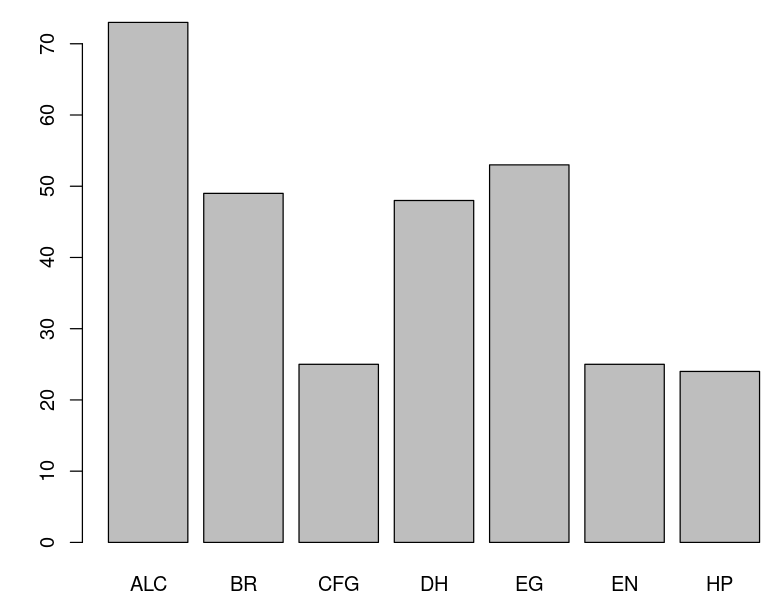
\includegraphics{img/barplot(table).png}

\begin{enumerate}
\def\labelenumi{\arabic{enumi}.}
\setcounter{enumi}{21}
\tightlist
\item
  Boite à moustache des notes de final
\end{enumerate}

\begin{Shaded}
\begin{Highlighting}[]
\KeywordTok{boxplot}\NormalTok{(X}\OperatorTok{$}\NormalTok{final)}
\end{Highlighting}
\end{Shaded}

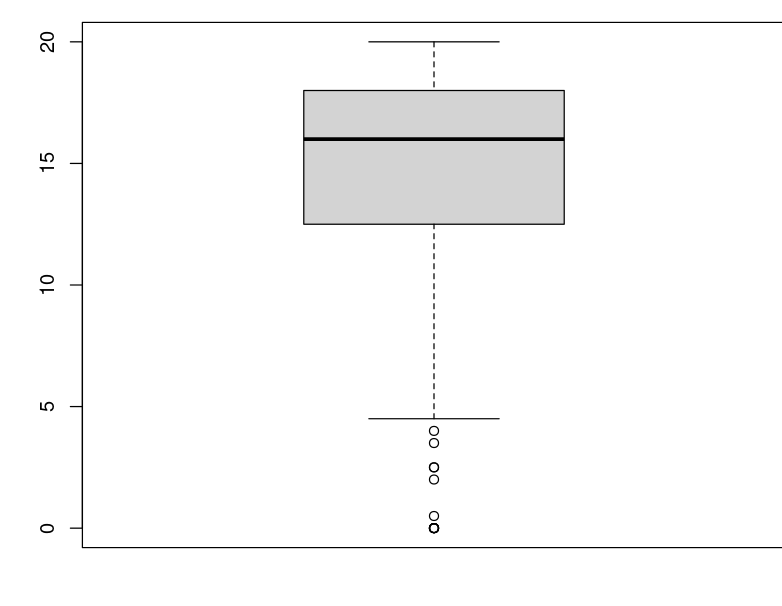
\includegraphics{img/boxplot(final).png}

\begin{enumerate}
\def\labelenumi{\arabic{enumi}.}
\setcounter{enumi}{22}
\item
  TODO : ?
\item
  Diagramme en tige et feuille de la moyenne
\end{enumerate}

\begin{Shaded}
\begin{Highlighting}[]
\KeywordTok{stem}\NormalTok{(X}\OperatorTok{$}\NormalTok{moyenne)}
\end{Highlighting}
\end{Shaded}

\begin{verbatim}
   0 | 224
   1 | 247
   2 | 3
   3 | 22
   4 | 79
   5 | 0124469
   6 | 01134579
   7 | 02457
   8 | 22355888
   9 | 2224
  10 | 1255
  11 | 000111223345899
  12 | 0000001112233335555566667777788999
  13 | 00022234455666667777
  14 | 00000111223333344455666666778889999
  15 | 000001222333444455566666666677889999
  16 | 00011122333333455556667777788999
  17 | 000011122333444444456667888999
  18 | 00000011122223444566788899999
  19 | 00011223333444678
  20 | 00
\end{verbatim}

\begin{enumerate}
\def\labelenumi{\arabic{enumi}.}
\setcounter{enumi}{24}
\tightlist
\item
  Histogramme des notes du final
\end{enumerate}

\begin{Shaded}
\begin{Highlighting}[]
\KeywordTok{hist}\NormalTok{(X}\OperatorTok{$}\NormalTok{final)}
\end{Highlighting}
\end{Shaded}

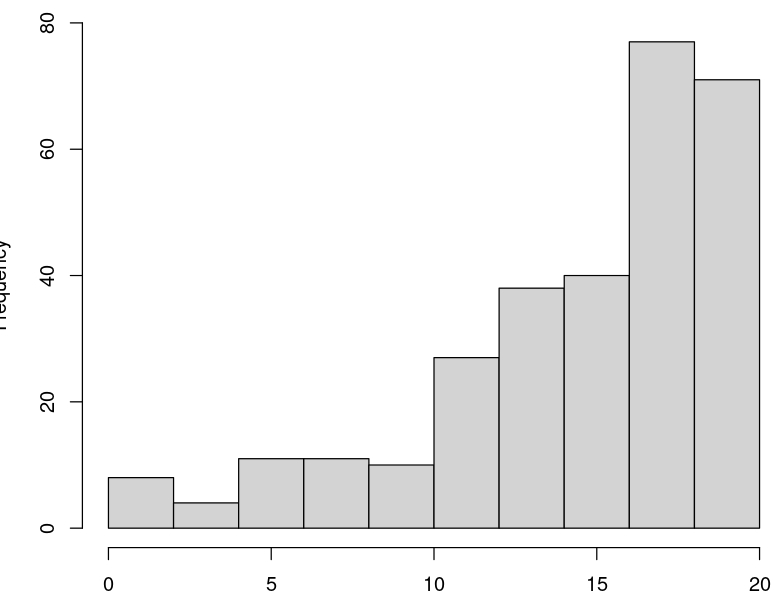
\includegraphics{img/hist(final).png}

\begin{enumerate}
\def\labelenumi{\arabic{enumi}.}
\setcounter{enumi}{25}
\tightlist
\item
  Coupe l'histogramme à 15
\end{enumerate}

\begin{Shaded}
\begin{Highlighting}[]
\KeywordTok{hist}\NormalTok{(X}\OperatorTok{$}\NormalTok{final, }\DataTypeTok{breaks =} \KeywordTok{c}\NormalTok{(}\DecValTok{0}\NormalTok{,}\DecValTok{15}\NormalTok{,}\DecValTok{20}\NormalTok{))}
\end{Highlighting}
\end{Shaded}

\begin{enumerate}
\def\labelenumi{\arabic{enumi}.}
\setcounter{enumi}{26}
\item
  TODO
\item
  TODO
\item
\end{enumerate}

\begin{Shaded}
\begin{Highlighting}[]
\KeywordTok{plot}\NormalTok{(X}\OperatorTok{$}\NormalTok{median , X}\OperatorTok{$}\NormalTok{final)}
\end{Highlighting}
\end{Shaded}

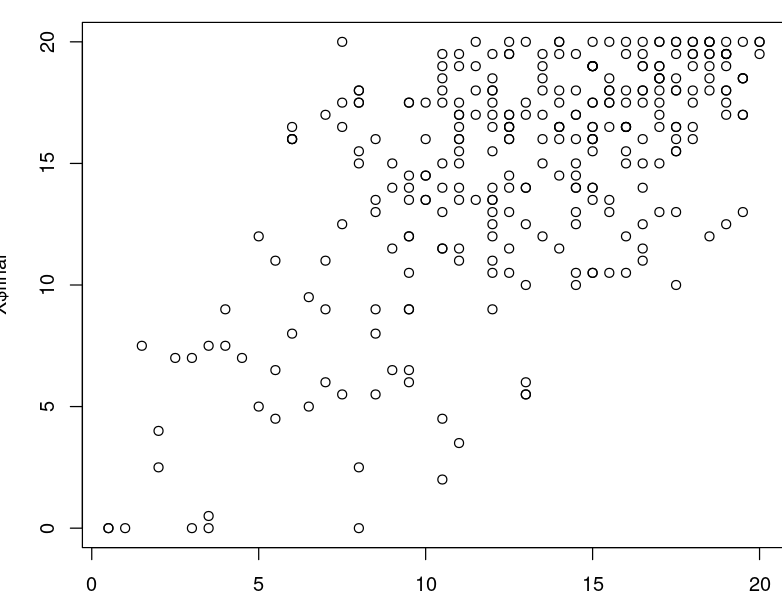
\includegraphics{img/plot.png} On remarque que les valeurs sont dans la
diagonale. Les notes du médian et du final sont donc un peu près égales
pour tout les étudiants : Un étudiant qui réussi le final réussi aussi
le médian et inversement.

\begin{enumerate}
\def\labelenumi{\arabic{enumi}.}
\setcounter{enumi}{29}
\tightlist
\item
  Boite à moustache en fonction des correcteurs
\end{enumerate}

\begin{Shaded}
\begin{Highlighting}[]
\KeywordTok{boxplot}\NormalTok{(X}\OperatorTok{$}\NormalTok{final }\OperatorTok{\textasciitilde{}}\StringTok{ }\NormalTok{X}\OperatorTok{$}\NormalTok{correcteur.final) }\CommentTok{\# Boite à moustache en fonction des correcteurs}
\end{Highlighting}
\end{Shaded}

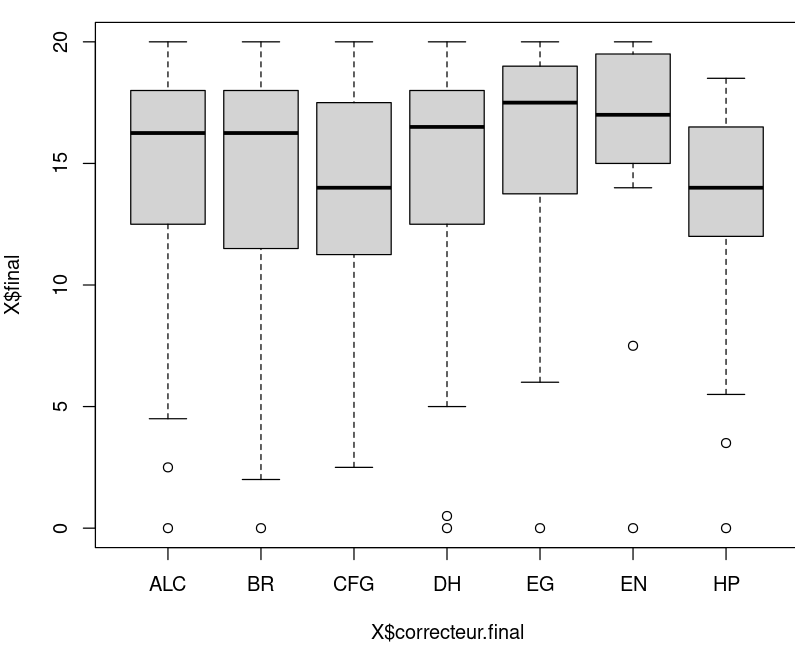
\includegraphics{img/boxplot(double).png}

\begin{enumerate}
\def\labelenumi{\arabic{enumi}.}
\setcounter{enumi}{30}
\tightlist
\item
  Boite à moustache du correcteur DH
\end{enumerate}

\begin{Shaded}
\begin{Highlighting}[]
 \KeywordTok{boxplot}\NormalTok{(X}\OperatorTok{$}\NormalTok{final[X}\OperatorTok{$}\NormalTok{correcteur.final }\OperatorTok{==}\StringTok{ "DH"}\NormalTok{] }\OperatorTok{\textasciitilde{}}\StringTok{ }\NormalTok{X}\OperatorTok{$}\NormalTok{correcteur.final[X}\OperatorTok{$}\NormalTok{correcteur.final }\OperatorTok{==}\StringTok{ "DH"}\NormalTok{])}
\end{Highlighting}
\end{Shaded}

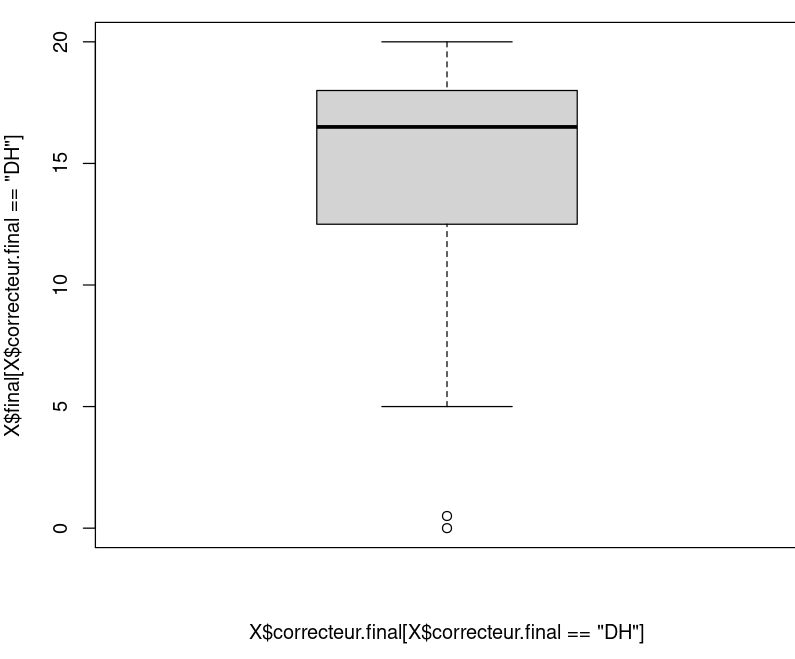
\includegraphics{img/boxplot(DH).png}

\begin{enumerate}
\def\labelenumi{\arabic{enumi}.}
\setcounter{enumi}{31}
\tightlist
\item
  Graph avec les carrés
\end{enumerate}

\begin{Shaded}
\begin{Highlighting}[]
\KeywordTok{stripchart}\NormalTok{(X}\OperatorTok{$}\NormalTok{final }\OperatorTok{\textasciitilde{}}\StringTok{ }\NormalTok{X}\OperatorTok{$}\NormalTok{correcteur.final, }\DataTypeTok{data =}\NormalTok{ X)}
\end{Highlighting}
\end{Shaded}

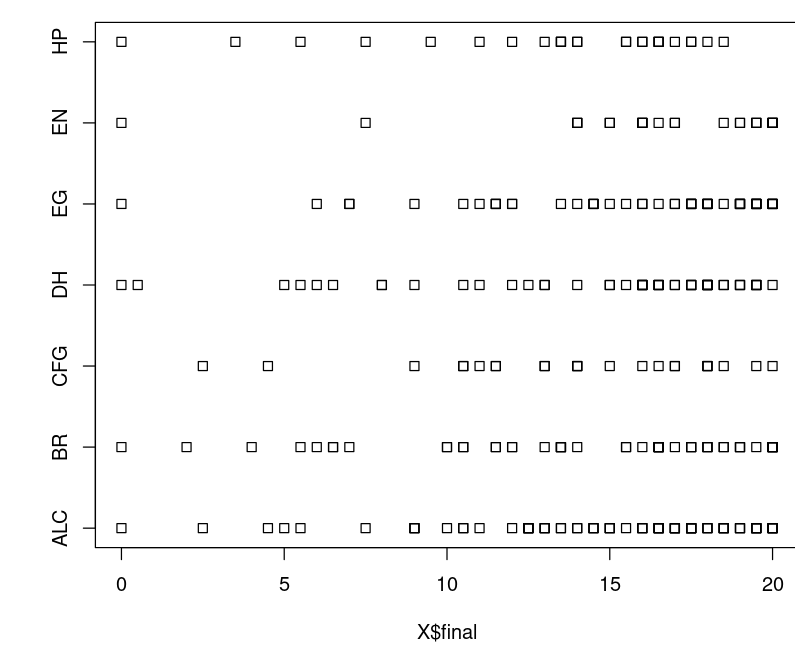
\includegraphics{img/stripchart.png}

\begin{enumerate}
\def\labelenumi{\arabic{enumi}.}
\setcounter{enumi}{32}
\tightlist
\item
  \(method = "jitter"\) permet de décaler les carrés pour mieux voir le
  nombre de points présents
\end{enumerate}

\begin{Shaded}
\begin{Highlighting}[]
\KeywordTok{stripchart}\NormalTok{(X}\OperatorTok{$}\NormalTok{final }\OperatorTok{\textasciitilde{}}\StringTok{ }\NormalTok{X}\OperatorTok{$}\NormalTok{correcteur.final, }\DataTypeTok{data =}\NormalTok{ X, }\DataTypeTok{method =} \StringTok{"jitter"}\NormalTok{)}
\end{Highlighting}
\end{Shaded}

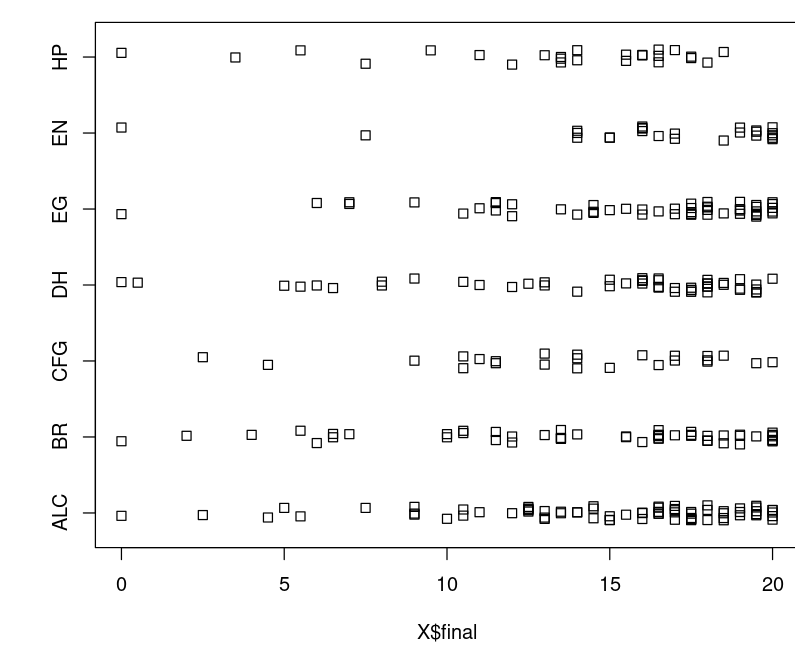
\includegraphics{img/stripchart(jitter).png}

\end{document}
